The dataset for this experiment was created on the bases of the dataset of noise free images. Just like before it contained various images with regions in different shades of red, green and blue. In each image there was one red object in a green neighbourhood that could have a shape of square, circle or letter H. Original images and those presenting expected results were exactly the same as in case of noise-free images. The different between those two datasets lies in images with a reduced colour palette as for the described experiment these images were subjected to the process of random addition of noise. For each image from training, validation and testing sets that was obtained by colour quantisation process, there was a 40\% chance of wrong colour assignment. For example a superpixel that has a bluish colour in an original image can be represented by red or green colour in an image with a reduced colour palette. The number of noised superpixels was randomly chosen and varied from 1 to 20. Figure \ref{fig:nonlinear_testset_noised} presents the same five sample images as in case of noise-free data, however this time some superpixels from an original image have a different colour assigned in images after colour quantisation. 

\begin{figure}[!htb]
 \centering
    \begin{tabular}{ccc}
        \textit{original image} & \textit{colour quantisation} & \textit{ground truth} \\
        \fcolorbox{black}{white}{\includegraphics[width= 0.22\textwidth]{nonlinear_noised/init/3.png}} &
        \fcolorbox{black}{white}{\includegraphics[width = 0.22\textwidth]{nonlinear_noised/test/3.png}} &
        \fcolorbox{black}{white}{\includegraphics[width = 0.22\textwidth]{nonlinear_noised/result/3.png}} \\
        \fcolorbox{black}{white}{\includegraphics[width = 0.22\textwidth]{nonlinear_noised/init/5.png}} &
        \fcolorbox{black}{white}{\includegraphics[width = 0.22\textwidth]{nonlinear_noised/test/5.png}} &
        \fcolorbox{black}{white}{\includegraphics[width = 0.22\textwidth]{nonlinear_noised/result/5.png}} \\
        \fcolorbox{black}{white}{
\includegraphics[width = 0.22\textwidth]{nonlinear_noised/init/6.png}} &
        \fcolorbox{black}{white}{
\includegraphics[width = 0.22\textwidth]{nonlinear_noised/test/6.png}} &
        \fcolorbox{black}{white}{
\includegraphics[width = 0.22\textwidth]{nonlinear_noised/result/6.png}} \\
        \fcolorbox{black}{white}{\includegraphics[width = 0.22\textwidth]{nonlinear_noised/init/9.png}} &
        \fcolorbox{black}{white}{\includegraphics[width = 0.22\textwidth]{nonlinear_noised/test/9.png}} &
        \fcolorbox{black}{white}{\includegraphics[width = 0.22\textwidth]{nonlinear_noised/result/9.png}} \\
        \fcolorbox{black}{white}{\includegraphics[width = 0.22\textwidth]{nonlinear_noised/init/13.png}} &
        \fcolorbox{black}{white}{\includegraphics[width = 0.22\textwidth]{nonlinear_noised/test/13.png}} &
        \fcolorbox{black}{white}{\includegraphics[width = 0.22\textwidth]{nonlinear_noised/result/13.png}} \\
    \end{tabular}
    \caption{Sample images generated for the problem of segmentation by shape on a noised images.}
    \label{fig:nonlinear_testset_noised}
\end{figure}

Noise on images reflect the whole probability distribution of features that is needed to compute the unary potential. Even if there are only few noised images versus few hundreds of noise-free images the segmentation method may perform much worse. The best way to explain why the accuracy of the method is so dependent on the presence of noise is to take as example a classification of green and blue regions. For noise-free images green regions are always labelled as \nth{1}, and blue as \nth{2} class. Given the fact that in the set of all available features there is a feature $k$ that represents the colour of a given superpixel, the  probability $p(f_{i,k}|y_i)$ for example for a blue superpixel will be equal to 100\% for label 2 and 0\% otherwise. Then, no matter what are the probabilities of other features, probability $p(f_i|y_i)$, and consequently the final probability $p(y_i|x_i)$ of a given label conditioned on the current superpixel will also be equal to 100\% for label 2, and 0\% for other labels. Hence, the labelling chosen by the unary potential for those two classes will always be perfect. On the other hand, for noised images, even if there are only few blue superpixels which do not have label 2, the probability $p(f_{i,k}|y_i)$ will be close to 0, but not equal to 0\%. Hence, probabilities of other features have a large influence on the final result, and as a result the final labelling may not be correct. Therefore, proper selection of features is crucial for the experiments on noised images.  

